\section{Material and methods}\label{sec:methods}

\subsection{Problem setting}\label{sec:problem}

We consider an operator that runs a set $\mathcal{S}$ of data-centre sites connected by a wide-area network. Time is divided into hourly slots $t=0,1,2,\dots$ Deferrable batch jobs arrive online. Job $j$ is released at the start of hour $a_j$ at origin site $o_j\in\mathcal{S}$. It carries $w_j$ server-hours of work made of independent tasks (a bag of tasks), can use at most $m_j$ servers concurrently, and must finish before the start of hour $d_j>a_j$. Work may be paused and resumed, and any part of it may run at a site other than its origin. Remote execution requires moving input data. At site $s$ and hour $t$, $K_s(t)$ servers are free for batch work once the interactive load has been served.

Let $I_s(t)$ be the average carbon intensity of the electricity supplied to site $s$ during hour $t$ (gCO$_2$/kWh). Executing one server-hour of job $j$ at site $s$ during hour $t$ emits
\begin{equation}\label{eq:unitcost}
c_{o_j s}(t) = e\,\mathrm{PUE}_s\, I_s(t) + \mathbf{1}[s\neq o_j]\,\delta\,\eta\,\tfrac{1}{2}\big(I_{o_j}(t)+I_s(t)\big),
\end{equation}
where $e$ is the IT energy per server-hour, $\mathrm{PUE}_s$ is the power usage effectiveness of site $s$, $\delta$ is the data volume moved per migrated server-hour and $\eta$ is the energy intensity of network transfer (kWh/GB). The transfer term charges network energy at the mean intensity of the two endpoints. With decision variables $x_{js}(t)\ge 0$ (server-hours of job $j$ run at site $s$ in hour $t$), the offline version of the problem is the linear programme
\begin{align}
\min_{x,u\ge 0}\quad & \sum_j\sum_{s}\sum_{t=a_j}^{d_j-1} c_{o_j s}(t)\,x_{js}(t) + \sum_j \Pi\, u_j \label{eq:obj}\\
\text{s.t.}\quad & \textstyle\sum_{s}\sum_{t=a_j}^{d_j-1} x_{js}(t) + u_j = w_j && \forall j, \label{eq:work}\\
& \textstyle\sum_{s} x_{js}(t) \le m_j && \forall j,\ t\in[a_j,d_j), \label{eq:width}\\
& \textstyle\sum_{j:\,a_j\le t<d_j} x_{js}(t) \le K_s(t) && \forall s,t, \label{eq:cap}
\end{align}
where $u_j$ is work left unfinished at the deadline and $\Pi$ is a lateness penalty much larger than any emission cost. When migration is not allowed, $x_{js}(t)=0$ for $s\neq o_j$. With complete knowledge of arrivals and intensities, the optimum of (\ref{eq:obj})--(\ref{eq:cap}) is a lower bound for every online policy, and we use it as the \emph{clairvoyant oracle}. An online scheduler has to fix $x_{\cdot s}(t)$ at the start of hour $t$. At that point it knows the jobs released so far, the current intensities $I_s(t)$ and nothing more than forecasts of $I_s(t+h)$ and of future arrivals.

\begin{proposition}[Network-flow structure]\label{prop:flow}
Problem (\ref{eq:obj})--(\ref{eq:cap}) is a minimum-cost flow problem on a network with a source, one node per job, one node per (job, hour) pair, one node per (hour, site) pair and a sink. Arc capacities are $w_j$ (source$\to j$), $m_j$ ($j\to(j,t)$) and $K_s(t)$ ($(t,s)\to$ sink). The only arcs with a cost are $(j,t)\to(t,s)$, priced at $c_{o_j s}(t)$, and a slack arc $j\to$ sink priced at $\Pi$.
\end{proposition}
\begin{proof}
Conservation at the job node is Eq.~(\ref{eq:work}). The capacity of arc $j\to(j,t)$ is Eq.~(\ref{eq:width}), conservation at $(j,t)$ splits that hour's work across sites, and the capacity of $(t,s)\to$ sink is Eq.~(\ref{eq:cap}). Conversely, every feasible flow defines a feasible $(x,u)$ with the same cost. The constraint matrix of the flow formulation is a node-arc incidence matrix, in which every column has exactly one $+1$ and one $-1$, so it is totally unimodular.
\end{proof}

Proposition~\ref{prop:flow} has a practical consequence. The oracle and every planning problem solved online (Section~\ref{sec:carma}) can be solved exactly by network simplex~\cite{ahuja1993network}, and integral data (work quantised to $0.01$ server-hours) give integral optimal flows. We use the OR-Tools implementation~\cite{ortools}. On the instances studied, network simplex returned the same objective value as a general-purpose LP solver (HiGHS) to within rounding, and it cut the total run time of the online planners by a factor of about six.

\subsection{Probabilistic carbon-intensity forecasting}\label{sec:forecast}

\paragraph{Point model} For each horizon $h=1,\dots,H$ ($H=24$ h) we fit a direct gradient-boosted regression tree model~\cite{friedman2001greedy} that predicts the change $I_s(t+h)-I_s(t)$ from information available at issue time $t$. Direct per-horizon models avoid the error accumulation of recursive strategies~\cite{taieb2012review}. One model per horizon is pooled across sites, with the site as a categorical feature. The features are the current intensity; differences between the current value and lags of 1, 2, 3, 6, 12 and 23 hours; the value observed at the same hour of the target on the previous day and in the previous week; a 24-hour rolling mean and mean absolute change (volatility); the national (GB) intensity; the regional wind, solar and gas shares; and calendar encodings of the target time (hour of day, day of week, annual sine and cosine). Models are fitted with absolute-error loss, so they estimate the conditional median. We use scikit-learn's histogram gradient boosting~\cite{pedregosa2011scikit} with 400 iterations, learning rate 0.05, 31 leaves and at least 50 samples per leaf. The models use only information available when the forecast is issued, and no weather forecasts. This is deliberate: the goal is a forecaster any operator can build from a public intensity feed.

\paragraph{Conformal upper quantiles} A point forecast $\hat I_s(t+h\,|\,t)$ is turned into calibrated upper quantiles by split conformal prediction~\cite{vovk2005algorithmic,lei2018distribution} with normalised scores. On a calibration window disjoint from training, we compute for each site $s$ and horizon $h$
\begin{equation}
r_{s,h}(t) = \frac{I_s(t+h)-\hat I_s(t+h\,|\,t)}{\sigma_s(t)+\epsilon},
\end{equation}
where $\sigma_s(t)$ is the 24-hour mean absolute hourly change observed at issue time and $\epsilon=5$~gCO$_2$/kWh. For a target level $\beta$, the upper forecast is $U^{\beta}_s(t+h\,|\,t)=\hat I_s(t+h\,|\,t)+\hat q_{s,h}(\beta_{s,h}(t))\,(\sigma_s(t)+\epsilon)$, where $\hat q_{s,h}(\cdot)$ is the empirical quantile function of the calibration scores. Grid carbon intensity is not exchangeable over time: 2024 was markedly cleaner than 2022--2023 (Fig.~\ref{fig:data}). We therefore update the working level online by adaptive conformal inference (ACI)~\cite{gibbs2021adaptive}. Once $I_s(t+h)$ is observed,
\begin{equation}\label{eq:aci}
\alpha_{s,h} \leftarrow \alpha_{s,h} + \gamma\big((1-\beta) - \mathbf{1}[I_s(t+h) > U^{\beta}_s(t+h\,|\,t)]\big),\qquad \beta_{s,h}(t)=1-\alpha_{s,h},
\end{equation}
with step size $\gamma=0.005$. By the ACI result of~\cite{gibbs2021adaptive}, the long-run frequency with which realised intensities exceed $U^\beta$ converges to $1-\beta$ for any data sequence, with no distributional assumption. This matters for the scheduler: the level $\beta$ becomes an interpretable risk dial, and it stays valid under drift. With $\beta=0.5$ the procedure also removes level shifts in the point model (a recalibrated median).

\subsection{CARMA: carbon-aware anticipatory receding-horizon multi-site allocation}\label{sec:carma}

A standard receding-horizon (model predictive control, MPC) scheduler~\cite{rawlings2017model} solves, at every hour $t$, the flow problem of Proposition~\ref{prop:flow} restricted to pending jobs and the window $[t,t+H)$. Future intensities are replaced by forecasts, and only the first hour of the plan is executed. Such a planner is \emph{myopic about demand}: it sees only jobs that have already arrived. The next result shows that this can be arbitrarily costly even when carbon intensities are known exactly.

\begin{proposition}[Myopia can be unboundedly costly]\label{prop:myopic}
Even with perfect intensity forecasts, myopic receding-horizon scheduling has no finite competitive ratio with respect to the clairvoyant oracle.
\end{proposition}
\begin{proof}
Take a clean site $A$ with one server and a dirty site $B$ with ample capacity. Let $c_A(0)=\varepsilon$, $c_A(1)=0$ and $c_B(0)=c_B(1)=c$, and ignore transfer costs. A flexible job ($w=1$, $m=1$) arrives at $t=0$ with deadline $d=2$. An urgent job ($w=1$) arrives at $t=1$ with $d=2$. At $t=0$ the myopic planner sees only the flexible job and defers it to $A$ at $t=1$ (cost $0<\varepsilon$). At $t=1$ both jobs must run in the same hour, one of them at $B$, so the total cost is $c$. The oracle runs the flexible job at $t=0$ and the urgent job at $t=1$, both at $A$, for a total of $\varepsilon$. The ratio $c/\varepsilon$ is unbounded as $\varepsilon\to 0$.
\end{proof}

The mechanism in Proposition~\ref{prop:myopic} is common in practice. Low-carbon capacity is scarce, and a myopic planner spends it on flexible work that could have waited or run elsewhere, leaving urgent jobs that arrive later to run on carbon-intensive capacity. CARMA addresses it by anticipating demand inside the same flow problem, and optionally prices forecast risk.

\begin{figure}[t]
\centering
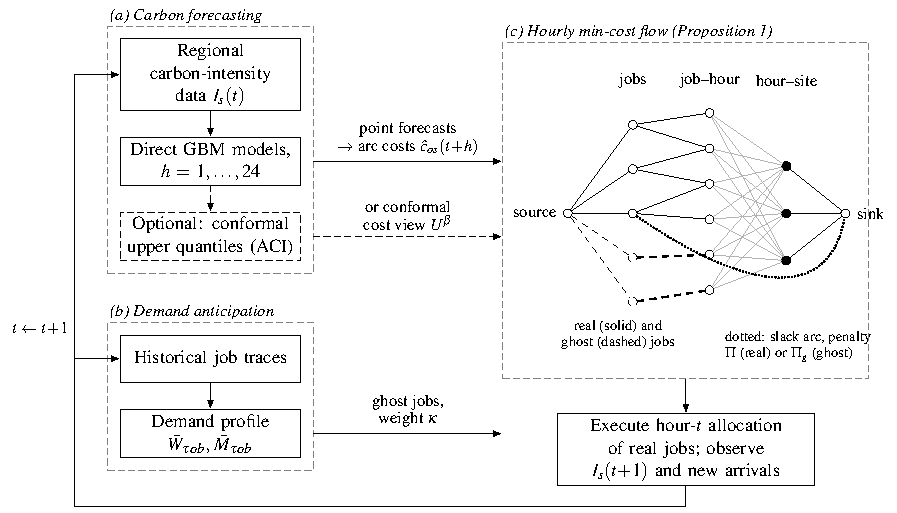
\includegraphics[width=\textwidth]{../figures/fig1_carma.pdf}
\caption{The CARMA decision loop. (a) Probabilistic carbon-intensity forecasts price the job--hour to hour--site arcs. (b) A demand profile learned from past traces generates ghost jobs for expected arrivals. (c) Real jobs (solid) and ghost jobs (dashed) share one min-cost flow network, whose dotted slack arc carries unfinished work to the sink at the lateness penalty. The network is solved exactly every hour, and only the first-hour allocation of real jobs is executed.}
\label{fig:carma}
\end{figure}

\paragraph{Anticipated demand (ghost jobs)} From the operator's own history we estimate, for every hour of the week $\tau$, origin $o$ and window class $b$, the expected work $\bar W_{\tau ob}$ and the expected total width $\bar M_{\tau ob}$ of arriving jobs. Window classes are the bins $\mathcal{B}=\{1,2,4,6,9,13,18,24\}$ hours. A job is assigned to the largest bin not exceeding its window, so ghost jobs are never more flexible than the jobs they represent. At hour $t$, for each $k=1,\dots,\ell$ (the look-ahead), CARMA adds to the planning problem a \emph{ghost job} for every $(o,b)$ with work $\kappa\bar W_{\tau(t+k)ob}$, width $\kappa\bar M_{\tau(t+k)ob}$, release $t+k$ and deadline $\min(t+k+b,\,t+H)$. Ghost jobs compete with real jobs for capacity, but their slack arc is priced at a moderate penalty $\Pi_g$, set to $1.5$ times the largest local unit cost in the window, rather than at $\Pi$. They can therefore reserve clean capacity when it is economical but never force real work to be late. The weight $\kappa\ge 0$ scales how much of the expected demand is anticipated. With $\kappa=0$, CARMA reduces to myopic MPC.

\paragraph{Carbon cost view} Future-hour costs in Eq.~(\ref{eq:unitcost}) are evaluated at a forecast of $I_s(t+h)$; for the current hour ($h=0$) the observed intensity is used. CARMA admits two cost views: the point forecast $\hat I$, or the conformal upper quantile $U^{\beta}$ of Section~\ref{sec:forecast}. The second is motivated by the optimizer's curse~\cite{smith2006optimizer}: selecting the minimum over noisy estimates is biased towards optimism, and a level $\beta>0.5$ penalises uncertain future hours in proportion to their calibrated spread. Whether this risk premium helps is an empirical question, and we treat the cost view as a hyperparameter.

\paragraph{Algorithm} Fig.~\ref{fig:carma} summarises the loop. At each hour $t$, CARMA (i) observes $I_s(t)$, the free capacity and the pending jobs; (ii) builds the cost cube $c_{os}(t+h)$ for $h<H$ from the chosen forecast view; (iii) adds the ghost jobs for hours $t+1,\dots,t+\ell$; (iv) solves the resulting min-cost flow problem exactly; (v) executes the first-hour allocations of the real jobs only; and (vi) after observing the realised intensities, updates the ACI levels by Eq.~(\ref{eq:aci}) when conformal costs are used. Overdue work gets a one-hour window and is served with priority. The planning network has $O\big((n_t+\ell|\mathcal{S}||\mathcal{B}|)\,H\,|\mathcal{S}|\big)$ arcs, where $n_t$ is the number of pending jobs, so each decision takes a few tens of milliseconds (Section~\ref{sec:results}). The hyperparameters $(\kappa,\ell)$ and the cost view are tuned on validation weeks that precede the test period (Section~\ref{sec:tuning}).

\subsection{Baselines}\label{sec:baselines}

We compare CARMA with the following online policies and the oracle. \textbf{ASAP-Local} is carbon-agnostic: it runs work at its origin as soon as possible, earliest deadline first (EDF). \textbf{Greedy-Spatial} also runs work immediately, but at the site that is currently cleanest; this is geographical load balancing without temporal shifting~\cite{liu2011greening}. \textbf{Forecast-Reserve} books, when a job arrives, the cheapest forecast (site, hour) slots in its window that still have capacity, and never revises the booking. This is the lowest-window strategy of~\cite{wiesner2021lets} extended to multiple sites. \textbf{MPC} is the myopic receding-horizon flow scheduler with point forecasts. \textbf{MPC+conformal} uses the conformal upper quantile at the level that was best for MPC on validation data. \textbf{MPC-Perfect} is MPC given the realised intensities, which isolates the value of forecast accuracy. \textbf{CARMA-Perfect} is CARMA given the realised intensities, and \textbf{CARMA+conformal} is CARMA with the best conformal cost view. \textbf{Oracle} solves (\ref{eq:obj})--(\ref{eq:cap}) with full knowledge of arrivals and intensities.

\subsection{Data and experimental design}\label{sec:data}

\paragraph{Carbon intensity} We use half-hourly regional carbon intensity for Great Britain from the Carbon Intensity API of the National Energy System Operator (NESO)~\cite{nesoapi} from 1 January 2022 to 31 December 2024. Values are averaged to hourly resolution. Four regions host the candidate sites: South Scotland, North West England, West Midlands and London. They span the north--south gradient of the British grid, from wind- and nuclear-rich South Scotland to gas-dependent London, and include the main data-centre markets of London, Manchester (North West England) and Birmingham (West Midlands). Gaps (602 of 26{,}304 hours in at least one region) were filled by linear interpolation. The period up to 30 June 2023 is used to train the forecaster, July--September 2023 to calibrate the conformal scores, October--December 2023 to tune the scheduler, and all 52 weeks starting on Mondays in 2024 as the out-of-sample test set.

\paragraph{Sites and energy parameters} Batch capacities are 300, 400, 400 and 600 servers for South Scotland, North West England, West Midlands and London. This reflects a small, clean northern site and a large site in London. Interactive load takes $20\%\pm15\%$ of each site's capacity on a diurnal cycle that peaks in the afternoon. We assume $e=0.4$~kWh per server-hour. The assumed PUE values are 1.15, 1.20, 1.25 and 1.30 from north to south, reflecting free-cooling potential. Migrated work moves $\delta=2$~GB per server-hour at $\eta=0.02$~kWh/GB. This value lies within the wide range of published estimates of transmission energy intensity~\cite{aslan2018electricity}. We vary $\eta$ in a sensitivity analysis.

\paragraph{Workloads} Job arrivals follow a non-homogeneous Poisson process with a diurnal peak in the afternoon and 30\% lower weekend rates. Jobs originate at the four sites with probabilities 0.10, 0.20, 0.25 and 0.45. Width $m_j$ is log-uniform on $[4,64]$ servers and the run time at full width $r_j$ is uniform on $\{1,\dots,6\}$ hours, so $w_j=m_jr_j$. A share $\upsilon$ of jobs is urgent (deadline $=a_j+r_j$, no temporal slack); for the others the window is $\lceil f_j r_j\rceil$ hours with $f_j\sim U[1.5,4]$, capped at 24 hours. The baseline value is $\upsilon=0.3$. The arrival rate is scaled so that the offered load equals a fraction $\rho\in\{0.3,0.5,0.7\}$ of the mean free capacity. Each test episode covers one week of arrivals. We also simulate 24 hours of arrivals before and after the week, so the evaluated week starts and ends under steady-state congestion. Metrics are computed only for jobs released during the week. For each week and load level we draw one workload trace with a fixed seed, and every policy runs on that same trace. The demand profile used by CARMA is estimated from 13 independent historical traces. We study two regimes: \emph{spatio-temporal}, where migration is allowed, and \emph{temporal-only}, where it is not.

\paragraph{Metrics and statistics} The primary metric is operational emissions (tCO$_2$) per week. We report the reduction relative to ASAP-Local and the optimality gap relative to the oracle, the share of work finished late, the share of work executed away from its origin, and the decision time. Policies are compared by paired two-sided Wilcoxon signed-rank tests over the 52 test weeks, with Holm correction across comparisons.
